%! suppress = MissingLabel

Рассмотрим самую вершину башни интерпретаторов.
Там интерпретируется программа, которая сама по себе уже не является интерпретатором, а представляет собой API или UI запрос от внешнего мира.
Эта программа интерпретируется в некоторое преобразование данных $d_{in}\rightsquigarrow d_{out}$, которые в свою очередь уже не являются программой (поскольку им не даётся семантика).
Как выглядят эти преобразования, как их композиционно описывать?

\[
    d_{out} =
    U^{App}\left(
    \left<
    U_{App}^{API/UI},
    \left<
    p_{API/UI},
    d_{in}
    \right>
    \right>
    \right)
\]

Решением является \vocab{функциональная оптика}.
Она позволяет фокусироваться на некоторые свойства объекта и персистентно восстанавливать целый объект с новым значением свойств.
Разные средства фокусировки классифицируют как различные \vocab{оптические девайсы} по интерфейсу использования.
Например, линза может фокусироваться на знак числа, позволяя его просматривать и устанавливать.
Это свойство имеет тип \mintinline{haskell}|Bool|:
\begin{minted}{haskell}
    sign :: Lens' Int Bool
\end{minted}

Существует множество библиотек оптики как для Haskell\footnote{\url{https://hackage.haskell.org/package/optics-0.1/docs/Optics.html}}\footnote{\url{http://lens.github.io/}}\footnote{\url{https://github.com/marcosh/existential-optics/tree/main}}, так и для других языков: Kotlin\footnote{\url{https://arrow-kt.io/}}, Scala\footnote{\url{https://github.com/optics-dev/Monocle}}, Swift\footnote{\url{https://github.com/swiftlang/swift-evolution/blob/main/proposals/0161-key-paths.md}} (языковая поддержка).

\subsection{Персистентные структуры данных}

Структуры данных разделяют на \vocab{изменяемые (mutable)} и \vocab{неизменяемые (immutable)}.
Это классификация лишь по внутренней реализации, используются изменяемые ячейки памяти или нет.

По использованию выделают \vocab{эфемерные} и \vocab{персистентные} структуры данных.
После работы с эфемерной структурой, по той же ссылке может быть доступна другая структура.
\begin{minted}{kotlin}
    let xs = emptyMutableList<Int>()
    xs.add(42)
    print(xs)
\end{minted}

Работа с персистентными структурами порождает каждый раз новые ссылки, в то время как по старым доступна изначальная структура.
\begin{minted}{haskell}
    let xs = []
    let xs' = 42 : xs
    print xs'
\end{minted}

Может показаться, что эфемерные являются изменяемыми, а персистентные --- неизменяемыми.
На самом деле это более-менее ортогональные классификации.
Так, с помощью копирования можно к изменяемой структуре данных предоставить персистентный интерфейс, а неизменяемой --- эфемерный (с помощью монады \mintinline{haskell}|State|).

В речи, когда говорят о персистентных структурах данных, часто имеют в виду структуры данных с персистентным интерфейсом, специально оптимизированные для него (не требуют полного копирования на каждую операцию).
Способы построения таких структур и работы с ними на удивление довольно оптимальны и разнообразны~\cite{okasaki1999purely}.

Например, можно реализовать эффективный персистентный массив с логарифмической сложностью всех операций.
В Haskell такой структурой данных является \mintinline{haskell}|Seq|\footnote{\url{https://hackage.haskell.org/package/containers-0.7/docs/Data-Sequence.html}}\footnote{\url{http://www.staff.city.ac.uk/~ross/papers/FingerTree.html}}.
Если в вершинах хранить небольшие массивы, которые современные аритектуры процессоров могут эффективно копировать, можно существенно уменьшить высоту дерева и алгоритмическую сложность операций (e.g. \mintinline{scala}|scala.immutable.Vector|).

\begin{task}
    Реализуйте не Haskell персистентное декартово дерево по неявному ключу.
    Какие особенности Haskell усложняют использование этой структуры?
\end{task}

Когда использовать эфемерные, а когда персистентные структуры данных?
Если сравнивать, то можно обнаружить, что эфемерные можно реализовывать эффективнее во многих случаях, так как память изменяемая и кеши процессоров лучше работают с локальными данными (в то время как персистентные структуры обречены быть деревьями, чтобы реаллоцировать не структуру целиком, а только путь до корня).

Персистентные структуры же позволяют писать более модульный и безопасный с точки зрения многопоточности код, который может не учитывать возможность изменения структуры по ссылке.
В то время как работа с эфемерной структурой не является чистым кодом, а включает в себя порождение побочных эффектов.
Также объединение персистентными результатов разных вызовов может быть дешевле, как, например, конкатенация персистентных массивов дешевле конкатенации эфемерных (логарифмическая сложность против линейной).

Таким образом, в рамках ограниченного, легко обозреваемого скоупа лучше использовать эфемерные структуры ввиду их эффективности (например, чтобы изначально заполнить коллекцию элементами).
Однако, через границы абстракции лучше пропускать только персистентные структуры (или же положиться на систему эффектов, см.~\ref{sec:effect-systems}).
То есть каждая структура данных должна поддерживать две фазы своей жизни.
Например, так сделано в Scala, где у многих персистентных коллекций есть \mintinline{scala}|Builder| версия.

\subsection{Простейшая оптика}

Линзы являются простейшим примером оптического девайса.
Они позволяют гарантированно обозревать одно свойство и устанавливать его.

Изначально линзы были предложены как решение проблемы view-update в базах данных~\cite{bohannon2006relational, foster2008quotient}.
А именно --- как нужно изменить реальную базу при изменении view.
Или как восстанавливать целое после извлечения и изменения части.
Линзы тут являются средством двустороннего программирования --- позволяют одновременно описывать как view, так и способ обновления.

Параллельно\footnote{\url{https://github.com/ekmett/lens/wiki/History-of-Lenses}}, линзы упоминаются в серии блог-постов, описывающих попытку удобнее работать с изменяемым состоянием при написании игр\footnote{\href{https://web.archive.org/web/20140402193032/https://lukepalmer.wordpress.com/2007/07/26/making-haskell-nicer-for-game-programming/}{(post) Making Haskell nicer for game programming}}\footnote{\href{https://web.archive.org/web/20120303223802/https://lukepalmer.wordpress.com/2007/08/05/haskell-state-accessors-second-attempt-composability/}{(post) Haskell State Accessors (second attempt: Composability)}} (линзы в играх продолжают радовать\footnote{\url{http://www.timphilipwilliams.com/posts/2019-07-25-minecraft.html}}).

\subsubsection{Линзы --- costate coalgebra comonad}

% todo картинки

Простейшую линзу образуют пара функций --- просмотр и установка свойства:
\begin{minted}{haskell}
    data SimpleLens' s a = SimpleLens'
      { view' :: s -> a
      , set' :: s -> a -> s
      }
\end{minted}

На эти функции накладываются естественные законы:
\begin{minted}{haskell}
    view l (set l s x) ?$\equiv$? x
    set l s (view l s) ?$\equiv$? s
    set l (view l s x) y ?$\equiv$? set l s y
\end{minted}

Линзы можно композировать и обращаться к вложенным полям произведений.
Так, они могут быть морфизмами в категории типов.
При таком определении, правда, композиция работает в обратном, от желаемого, порядке.
\begin{minted}{haskell}
    instance Category SimpleLens' where
      id :: SimpleLens' s s
      id = SimpleLens' { view' = id, set' = flip const }

      (.) :: SimpleLens' a b -> SimpleLens' s a -> SimpleLens' s b
      l1 . l2 = SimpleLens'
        { view' = view' l1 . view' l2
        , set' = \s x -> set' l2 s (set' l1 (view' l2 s) x)
        }
\end{minted}

Например, можно легко изменить возраст пользователя:
\begin{minted}{haskell}
    newtype Age = Age { _getAge :: Int }
    data User = User { _userName :: String, _userAge :: Age }

    userAge :: SimpleLens' User Age
    userAge = SimpleLens' { view' = _userAge, set' = \s x -> s { _userAge = x } }

    getAge :: SimpleLens' Age Int
    getAge = SimpleLens' { view' = _getAge, set' = \s x -> s { _getAge = x } }

    ghci> set (getAge . userAge) user 1
\end{minted}

Можно обобщить линзы до полиморфных линз, которые позволяют пересоздавать структуру с новыми типовыми параметрами:
\begin{minted}{haskell}
    data SimpleLens s t a b = SimpleLens
      { view :: s -> a
      , set :: s -> b -> t
      }

    _1 :: SimpleLens (a, c) (b, c) a b
    _1 = SimpleLens { view = \(x, _) -> x, set = \(x, c) y -> (y, c) }
\end{minted}

Можно заметить, что линза в таком представлении является комонадой коалгеброй коstate\footnote{\href{https://youtu.be/9_iYlp8smc8?si=NLka0vnnhYDdTfgm}{(youtube) Category Theory II 9.1: Lenses.}}.
Действительно, пару функций можно заменить на функцию, возвращающую пару:
\begin{minted}{haskell}
    data Store a s = Store (a, a -> s)
    data DataLens s a = DataLens (s -> Store a s)
\end{minted}

Если определить инстанс комонады для \mintinline{haskell}|Store a s| и выписать законы совместимости с коалгеброй, мы получим в точности законы линз.

\subsubsection{Призмы}

Призмы позволяют получить свойство, которое может отсутствовать, и устанавливать его при наличии.
Так, конкретное поле типа-суммы может не удаться извлечь, при передаче не ожидаемого конструктора.

Простые призмы можно определить аналогично линзам, с учётом возможного отсутствия свойства:

\begin{minted}{haskell}
    data SimplePrism' s a = SimplePrism'
      { preview' :: s -> Maybe a
      , review' :: a -> s
      }
\end{minted}

Полиморфная призма должна предоставить структуру с обновлённым типом в случае неуспеха просмотра:
\begin{minted}{haskell}
    data SimplePrism s t a b = SimplePrism
      { preview :: s -> Either t a
      , review :: b -> t
      }
\end{minted}

Можно определить призму для работы с содержимым конструктора \mintinline{haskell}|Left|:
\begin{minted}{haskell}
    _Left :: SimplePrism (Either a c) (Either b c) a b
    _Left = SimplePrism
      { preview = \case Left a -> Right a; Right c -> Left (Right c)
      , review = Left
      }
\end{minted}

Композиция призм определяется естественным образом.

% todo сериализация это призма

\subsubsection{Композиция линз и призм}

Заведём класс типов, с помощью которого научимся композировать различные комбинации линз и призм.
Результирующий девайс однозначно определяется операндами композиции.

\begin{minted}{haskell}
    class Composable o1 o2 o3 | o1 o2 -> o3 where
      compose :: o1 s t a b -> o2 a b c d -> o3 s t c d
\end{minted}

Теперь можем естественным образом определить композицию для различных девайсов.
Можно заметить, что этот подход требует квадратичное количество инстансов от количества оптических девайсов.

\begin{minted}{haskell}
    instance Composable SimpleLens SimpleLens SimpleLens where
      compose :: SimpleLens s t a b -> SimpleLens a b c d -> SimpleLens s t c d
      compose l2 l1 = SimpleLens
        { view = view l1 . view l2
        , set = \s x -> set l2 s (set l1 (view l2 s) x)
        }
\end{minted}

Композиция линз и призм образует другой девайс --- аффинные траверсы, которые являются чем-то средним.
Наличие призмы в композиции не позволяет гарантированно просматривать свойство, а линзы --- создавать новое значение без изначального.
\begin{minted}{haskell}
    data AffineTraversal s t a b = AffineTraversal
      { apreview :: s -> Either t a
      , aset :: s -> b -> t
      }

    instance Composable SimplePrism SimpleLens SimplePrism where
      compose :: SimplePrism s t a b -> SimpleLens a b c d -> SimplePrism s t c d
      compose p l = SimplePrism
        { preview = fmap (view l) . preview p
        , pset = \s d -> case preview p s of
            Left t -> t
            Right a -> pset p s (set l a d)
        }
\end{minted}

% todo тут квадрат инстансов не нужен, нужно просто обоих к ближайшему предку апкастить

\subsection{Разнообразие оптических девайсов, \texttt{optics}} \label{subsec:optics}

Различных оптических девайсов можно придумать довольно много.
Библиотека \texttt{optics} предоставляет абстрактный интерфейс для самых популярных из них (рис.~\ref{fig:optics-hierarchy}).
Она имеет прекрасную документацию с подробным описанием девайсов\footnote{\url{https://hackage.haskell.org/package/optics-0.4.2.1/docs/Optics.html}}.

\begin{figure}
    \centering
    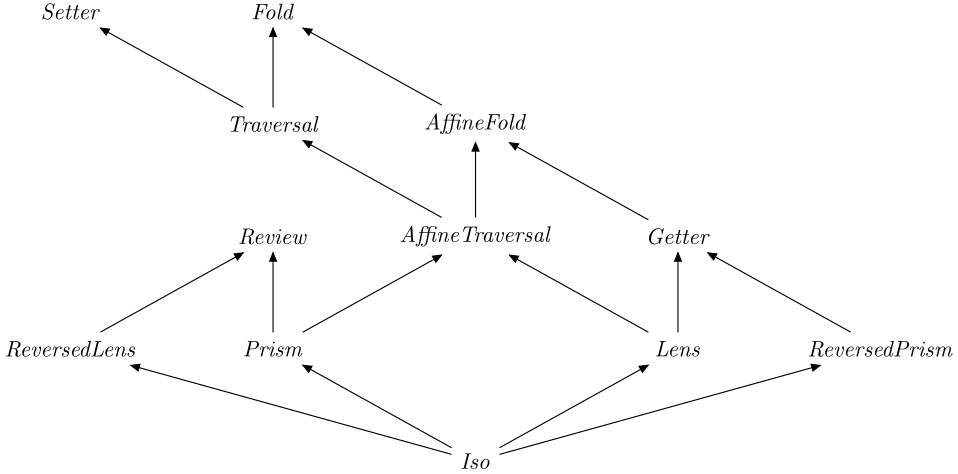
\includegraphics[width=\textwidth]{/home/yukio/Diary/projs/fpcourse/fp-2024/docs/figs/optics-hierarchy}
    \caption{Иерархия оптических девайсов \texttt{optics}.}
    \label{fig:optics-hierarchy}
\end{figure}

Примеры:
\begin{minted}{haskell}
    data Pet = Cat String | Dog Int deriving Show
    newtype UserName = UserName { _getUserName :: String } deriving Show
    data User = User { _userName :: UserName, _userCats :: [Pet] } deriving Show

    exampleUser :: User
    exampleUser = User (UserName "Bob") [Cat "Kitty", Dog 42, Dog 4]

    exampleName :: User -> User
    exampleName = over (userName % getUserName) (++ "!")

    exampleIx :: User -> User
    exampleIx = set (userName % getUserName % ix 2) 'k'

    exampleFold :: User -> Int
    exampleFold = getSum $ foldMapOf (userName % getUserName % folded) (const 1)

    examplePrint :: User -> IO User
    examplePrint = traverseOf (userCats % traversed % _Dog) (\x -> x <$ print x)
\end{minted}

\subsection{Другие представления оптики}

Ранее мы рассмотрели тривиальную оптику, составленную непосредственно из кортежа элиминирующих функций (пары разбора-пересборки значений).
Однако, у такого подхода есть существенные недостатки.
Во-первых, нужно определять много операций композиции для различных видов оптики.
То есть композиция девайсов --- что-то гораздо более сложное, чем композиция функций.
Во-вторых, это представление не очень эффективно, так как сложно представить, что компилятор будет инлайнить вызовы функций из структур данных.

Было приложено много усилий и теорката\footnote{\url{https://bartoszmilewski.com/category/lens/}}, чтобы получить другие представления оптики.
Некоторые из них являются просто одной функцией, кодирующей все нужные преобразования, а композиция определена как композиция таких функций.

\subsubsection{Semantic editor combinators}

TODO semantic editor combinators\footnote{\url{http://conal.net/blog/posts/semantic-editor-combinators}} % todo

\subsubsection{Линзы ван Лаарховена}

TODO van Laarhoven lens\footnote{\url{https://www.twanvl.nl/blog/haskell/cps-functional-references}}\footnote{\href{http://r6.ca/blog/20120623T104901Z.html}{(post) Polymorphic Update with van Laarhoven Lenses}} % todo

TODO lens\footnote{\url{http://lens.github.io/}} % todo

% todo uniplate

\subsubsection{Profunctor optics}

TODO % todo немножко profunctor optics

% todo ссылки на Бартоша

\subsubsection{Existential (coend) optics}

TODO\footnote{\url{https://github.com/marcosh/existential-optics/tree/main}}\footnote{\url{https://www.tweag.io/blog/2022-05-05-existential-optics/}}\footnote{\url{https://www.twanvl.nl/blog/haskell/isomorphism-lenses}}\footnote{\url{https://www.brunogavranovic.com/posts/2022-01-05-lenses-to-the-left-of-me.html}} % todo


\subsection{Генерация оптики}

Чтобы использовать оптику для работы со своими структурами данных, нужно так или иначе получить для них реализацию девайсов.

Некоторую специфичную оптику можно написать руками.
Например, позволяющую работать с нетривиальным свойством значения (знак числа, высота дерева\ldots).
Библиотеки предоставляют специальные билдеры, упрощающие конструирование\footnote{\url{https://hackage.haskell.org/package/optics-core-0.1/docs/Optics-Lens.html\#v:lens}}.

Некоторая оптика получается автоматически из инстансов стандартных классов типов.
Например, свёртки и траверсы\footnote{\url{https://hackage.haskell.org/package/optics-core-0.1/docs/Optics-Traversal.html\#g:6}}.
Дальше уже встаёт вопрос о генерации инстансов классов типов (см.~\ref{sec:datatype-generic}).

Поскольку линзы являются просто обобщением полей, а призмы --- конструкторов, их можно генерировать автоматически с помощью макросов по структуре данных\footnote{\url{https://hackage.haskell.org/package/optics-th-0.1/docs/Optics-TH.html}}.
Для этого используются конвенции, поля называются с подчёркиванием, а макрос сгенерирует линзы без подчёркивания.
С призмами наоборот.
Так, генерация для примера выше (\ref{subsec:optics}) будет выглядеть следующим образом:
\begin{minted}{haskell}
    makeLenses ''User
    makeLenses ''UserName
    makePrisms ''Pet
\end{minted}

TODO библиотека  % todo

TODO data-generic optics\footnote{\url{https://hackage.haskell.org/package/optics-core-0.4.1.1/docs/Optics-Label.html}}\footnote{\url{https://ghc.gitlab.haskell.org/ghc/doc/users_guide/exts/overloaded_record_update.html}}\footnote{\url{https://ghc.gitlab.haskell.org/ghc/doc/users_guide/exts/overloaded_labels.html}} % todo

TODO % todo


% todo библиотеки с оптикой для других языков

% todo transducers

% todo слайды Беляева

% todo zippers

% todo сравнение с datatype generic programming

% todo оптика как альтернатива стримам?

% todo first-class patterns should also be able to re-build the values that they match, Pattern Synonyms paper, кастомные паттерны это та же оптика только с фиксированной структурой, которая помогает с exhaustiveness

% todo data processing

% todo https://blog.poisson.chat/
% todo lens and serialization


% todo общее между оптикой и data-дженериками - нужно универсально работать с разными структурами, хоть они и все так или иначе суммы, например, мы это знаем. То есть вид структуры знаем, а конкретные конструкторы и прочее - нет.
